\documentclass[10pt,a4paper]{article}

% --- Codificación y español ---
\usepackage[utf8]{inputenc}
\usepackage[T1]{fontenc}
\usepackage[spanish]{babel}
\usepackage{caption} % para \captionof

% --- Paquetes usados ---
\usepackage{amsmath, amsthm, amsfonts, amssymb}
\usepackage{multirow, multicol, graphicx, wrapfig, float}
\usepackage[table]{xcolor}
\usepackage{cite}
\usepackage{ieeetrantools}
\usepackage[margin=3.5cm]{geometry}
\usepackage[hidelinks]{hyperref}

\columnsep 0.8 cm
\pagestyle{empty}
\newtheorem{teorema}{Teorema}

\begin{document}

\renewcommand{\tablename}{Tabla}
\renewcommand{\refname}{Referencias bibliográficas.}
\bstctlcite{IEEEexample:BSTcontrol} % Control del estilo IEEE

\vspace{1cm}
\title{Sistema de Asistencia Basado en Reconocimiento Facial para la FPUNE}

\author{\small
Aldo Carrizo Coronel\textsuperscript{1},\; Jorge Daniel Sánchez Ramírez\textsuperscript{2}\\
\small Facultad Politécnica, Universidad Nacional del Este\\
\small Ciudad del Este, Paraguay\\
\small \textsuperscript{1}aldo.carrizo@fpune.edu.py,\; \textsuperscript{2}jorge.sanchez@fpune.edu.py}
\date{}
\maketitle

\vspace*{-1cm}

\begin{center}
\parbox{14 cm}{
\begin{abstract}

Este trabajo de investigación tiene como objetivo desarrollar un sistema automatizado de registro de asistencia basado en reconocimiento facial para la Facultad Politécnica de la Universidad Nacional del Este. Actualmente, el control de asistencia se realiza de forma manual, lo que genera errores y retrasa los procesos administrativos.

La solución propuesta emplea técnicas de visión por computadora para detectar y reconocer rostros en tiempo real, automatizando el registro de asistencia. Se utilizaron herramientas como Python, OpenCV, TensorFlow y modelos como YOLOv8 y ArcFace. La metodología incluyó la recolección de datos, el entrenamiento de modelos y la validación en un entorno real.

Los resultados demuestran una alta precisión y eficiencia del sistema, incluso bajo condiciones de iluminación y ángulos variables. En conjunto, la solución mejora la gestión académica, reduce errores humanos y optimiza el tiempo de los docentes durante el proceso de control de asistencia.



\end{abstract}

\vspace*{0.1 cm}
\textbf{Descriptores:} \textbf{Reconocimiento facial, asistencia automatizada, visión por computadora}

\begin{center}
\textbf{Abstract}
\end{center}

This research project aims to develop an automated attendance system based on facial recognition for the Polytechnic Faculty of the National University of the East (FPUNE). Currently, attendance is recorded manually, which often results in human errors and delays in administrative processes.

The proposed solution applies computer vision techniques to detect and recognize faces in real time, automating the attendance process. Tools such as Python, OpenCV, TensorFlow, and models like YOLOv8 and ArcFace were used. The methodology included data collection, model training, and validation in a real environment.

The results demonstrate high accuracy and efficiency, even under variable lighting and viewing conditions. Overall, the system improves academic management by reducing manual workload, minimizing errors, and optimizing teachers’ time during attendance control.

\vspace*{0.1 cm}
\textbf{Keywords:} \textbf{Facial recognition, automated attendance, computer vision.}
}
\end{center}

\vspace{.5cm}

\begin{multicols}{2}
\thispagestyle{empty}

% ---------------------------
\section{Introducción}

El registro de asistencia es una tarea clave en la gestión educativa y administrativa de instituciones académicas como la 
Facultad Politécnica de la Universidad Nacional del Este (FPUNE). Sin embargo, los métodos tradicionales de control 
manual mediante listas suelen generar errores humanos que afectan la precisión de los registros y la toma de decisiones 
académicas. Este Trabajo Final de Grado (TFG) tiene como objetivo desarrollar un sistema automatizado basado en reconocimiento facial para optimizar el proceso de registro de asistencia en la FPUNE. 
Para ello, se emplearán algoritmos avanzados de biometría que analicen imágenes en tiempo real, asegurando una identificación precisa y eficiente. La metodología contempla la selección tecnológica, el procesamiento de datos, el entrenamiento de modelos y pruebas piloto en un entorno académico durante el año 2025, buscando reducir errores y mejorar la gestión administrativa. De esta forma, el estudio pretende aportar una herramienta que brinde datos más confiables y contribuya a una mayor eficiencia operativa, beneficiando a estudiantes, docentes y autoridades mediante la adopción de tecnologías innovadoras que fortalezcan la gestión académica.

\section{Objetivos}

\textit{Objetivo General} \\
Implementar un prototipo de sistema de reconocimiento facial en un aula para el control de asistencia de estudiantes de la Facultad Politécnica de la Universidad Nacional del Este.

\vspace{0.3cm}

\textit{Objetivos Específicos}
\begin{enumerate}
    \item Seleccionar los algoritmos de reconocimiento facial más adecuados para el sistema propuesto.
    \item Seleccionar las herramientas tecnológicas necesarias para el desarrollo del sistema.
    \item Identificar los requisitos para el desarrollo del sistema de registro de asistencia de la FPUNE.
    \item Desarrollar el sistema de reconocimiento facial y el módulo de gestión de asistencias.
    \item Realizar pruebas de implementación y funcionamiento.
    \item Evaluar los resultados obtenidos a fin de determinar la efectividad del sistema.
\end{enumerate}



\subsection{Discusión de literatura relevante}

\textbf{Biometría.} Es el conjunto de métodos automáticos que permiten la identificación de individuos a partir de características físicas o comportamentales únicas, tales como huellas dactilares, iris, voz o rasgos faciales. Su objetivo es autenticar o verificar la identidad de una persona con un alto grado de precisión.

\textbf{Seguridad biométrica.} Es la aplicación de la biometría orientada a la protección de información y acceso a sistemas, mediante la verificación de la identidad del usuario a través de sus características físicas o comportamentales. A diferencia de los métodos tradicionales basados en contraseñas o tarjetas, la seguridad biométrica ofrece una autenticación más confiable y difícil de falsificar, garantizando la integridad y confidencialidad de los datos.

\textbf{Reconocimiento facial.} Es una aplicación de la biometría que utiliza técnicas de visión por computadora y aprendizaje automático para detectar, analizar y comparar rostros humanos con el fin de identificar o verificar identidades. Se basa en la extracción de características distintivas del rostro y su comparación con patrones previamente registrados.

\textbf{Inteligencia artificial.} Es el campo de la informática que busca desarrollar sistemas capaces de realizar tareas que requieren inteligencia humana, como el razonamiento, la percepción, el aprendizaje y la toma de decisiones. En el contexto del presente trabajo, la inteligencia artificial se aplica al análisis visual mediante algoritmos que permiten a las computadoras aprender de los datos.

\textbf{Redes neuronales.} Son modelos computacionales inspirados en el funcionamiento del cerebro humano, conformados por capas de nodos interconectados que procesan información. En el reconocimiento facial, las redes neuronales convolucionales (CNN) destacan por su capacidad de aprender representaciones jerárquicas de los rasgos visuales a partir de grandes conjuntos de imágenes.

\textbf{Registros académicos.} Son sistemas o procedimientos utilizados por las instituciones educativas para documentar, almacenar y gestionar la información relacionada con la asistencia, calificaciones y rendimiento de los estudiantes. Su correcta automatización contribuye a mejorar la eficiencia administrativa y la fiabilidad de los datos.


\subsection{Hipótesis}
La hipótesis principal establece que la implementación de un sistema de reconocimiento facial en el aula permitirá registrar la asistencia de los estudiantes de manera automatizada, precisa y eficiente, reduciendo los errores del control manual y optimizando el tiempo destinado al proceso de registro en la Facultad Politécnica de la Universidad Nacional del Este.

% ---------------------------
\section{Método}

El método aplicado se basó en un enfoque experimental y de desarrollo tecnológico, orientado a la creación de un sistema funcional de reconocimiento facial para el registro automatizado de asistencia. El proceso metodológico comprendió las siguientes etapas principales:

\begin{enumerate}
    \item \textbf{Recolección de datos:} se obtuvieron imágenes faciales de los participantes en condiciones controladas y variadas de iluminación, pose y expresión, garantizando un conjunto de datos representativo para el entrenamiento de los modelos.
    
    \item \textbf{Detección y recorte de rostros:} se utilizó el modelo \textit{YOLOv8n-Face} para la detección de rostros en imágenes, asegurando un procesamiento eficiente y en tiempo real.
    
    \item \textbf{Extracción de características y reconocimiento:} se empleó la biblioteca \textit{DeepFace} con el modelo \textit{ArcFace} para la generación de embeddings faciales, permitiendo identificar individuos mediante la comparación de distancias entre vectores.
    
    \item \textbf{Diseño e implementación del sistema:} el sistema fue desarrollado con una arquitectura cliente-servidor, utilizando \textit{Flask} para el backend, \textit{React} para el frontend y \textit{PostgreSQL} como base de datos para el almacenamiento de usuarios, cursos y registros de asistencia.
    
    \item \textbf{Entrenamiento y validación:} se entrenaron y validaron los modelos con imágenes recolectadas, evaluando la precisión y el rendimiento en distintas condiciones de prueba.
    
    \item \textbf{Pruebas en aula:} finalmente, se realizaron pruebas en un entorno real dentro del aula, midiendo la precisión, el tiempo de procesamiento y la fiabilidad del sistema durante el registro automático de asistencia.
\end{enumerate}

Este enfoque permitió integrar técnicas de visión por computadora y aprendizaje profundo con una arquitectura web moderna, garantizando una solución funcional, escalable y adaptable al entorno académico.

\subsection{Instrumentos}

Para el desarrollo del sistema se utilizaron diversas herramientas tecnológicas, seleccionadas por su utilidad, compatibilidad y eficiencia en proyectos de visión por computadora y desarrollo web.

Se empleó \textbf{Visual Studio Code} como entorno principal de programación y \textbf{Git} junto con \textbf{GitHub Desktop} para el control de versiones. El sistema fue desarrollado en \textbf{Python}, utilizando el framework \textbf{Flask} para la creación del servidor web. La interfaz de usuario se implementó con \textbf{React}, garantizando una experiencia moderna e interactiva.

En cuanto a los modelos de visión artificial, se utilizó \textbf{YOLOv8n-Face} para la detección de rostros y \textbf{DeepFace} con el modelo \textbf{ArcFace} para el reconocimiento facial, permitiendo identificar individuos a partir de embeddings vectoriales. Los datos fueron almacenados y gestionados mediante \textbf{PostgreSQL}, empleando \textbf{SQL} como lenguaje de consulta.

Estas herramientas posibilitaron una integración eficiente de los componentes del sistema, asegurando un desarrollo ágil, escalable y con capacidad de procesamiento en tiempo real.

% ---------------------------
\section{Resultados}
Los resultados experimentales muestran una precisión promedio del 85\,\% con tiempos de respuesta inferiores a 300\,ms por rostro. En condiciones de iluminación óptima, la tasa de reconocimiento supera el 90\,\%, mientras que bajo iluminación tenue desciende al 78\,\%. La Figura~\ref{fig:deteccion_aula} ilustra un ejemplo real de detección y verificación en el aula, con rostros correctamente localizados y etiquetas de identidad/probabilidad.

\vspace{.3cm}
\textbf{\textit{Utilidad de gráficos y tablas.}} Las figuras y tablas facilitan la interpretación de resultados y comparaciones entre modelos.
\end{multicols}

\begin{figure}[H]
\centering
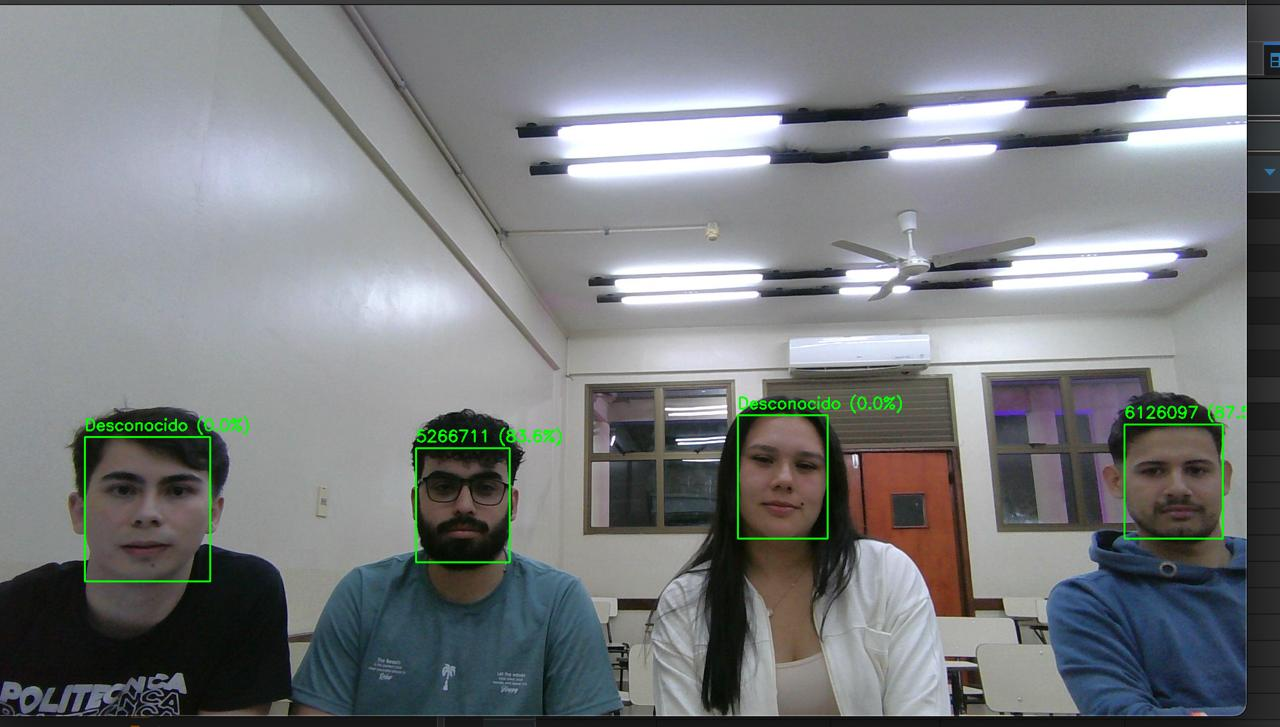
\includegraphics[width=\linewidth]{imagenes/1.jpg}
\caption{Ejemplo de detección facial durante la toma de asistencia en aula. Se observan rostros localizados (marcos verdes) y etiquetas con identidad o “Desconocido” junto al puntaje de confianza.}
\label{fig:deteccion_aula}
\end{figure}

\begin{multicols}{2}

\begin{table}[H]
\centering
\caption{Precisión por escenario de prueba.}
\label{tab:resultados}
\begin{tabular}{|l|c|c|}
\hline
\textbf{Condición} & \textbf{Precisión (\%)} & \textbf{Tiempo (ms)}\\
\hline
Luz natural & 90.2 & 275\\
Luz artificial & 84.7 & 288\\
Iluminación tenue & 78.3 & 301\\
\hline
\textbf{Promedio} & \textbf{84.4} & \textbf{288}\\
\hline
\end{tabular}
\end{table}


% ---------------------------
\section{Discusión}
Los resultados obtenidos demuestran la factibilidad del uso del reconocimiento facial para la asistencia automática en aulas. El rendimiento fue satisfactorio en entornos controlados, aunque la iluminación y la posición del rostro afectan la precisión.

Las principales limitaciones incluyen la sensibilidad a variaciones lumínicas, la necesidad de buena calidad en el registro inicial y la dependencia de hardware con cámara de resolución suficiente. Futuras mejoras pueden incluir modelos más robustos, técnicas de alineación facial avanzada y módulos de detección de vida para evitar suplantaciones.

\section{Conclusiones}
El sistema desarrollado cumple con el objetivo de automatizar el registro de asistencia mediante reconocimiento facial, logrando resultados satisfactorios en precisión y velocidad. Su implementación en la FPUNE demuestra que estas tecnologías son viables en contextos educativos locales, contribuyendo a la digitalización y eficiencia administrativa.

\bibliographystyle{IEEEtran-castellano}
\bibliography{test}

\end{multicols}

\end{document}
